% Choo Shop / choo-chu buyer, Round 3 architecture (week-08 midterm). Build: xelatex architecture.tex (pdflatex also works if kotex is installed)
% (page 2 is Korean through kotex; with xelatex/lualatex the Hangul font below is used instead)
% Fig. 1: processes and data flow. Fig. 2: the decision order inside one negotiation. Page 2: Korean notes.
% Grey = what the kit's default already has; blue = what this agent adds or replaces.
\documentclass[10pt]{article}
\usepackage[a4paper,landscape,margin=8mm]{geometry}
\usepackage{iftex}
\ifPDFTeX
  \usepackage{kotex}\newcommand{\hangulfont}{}
\else
  \usepackage{fontspec}
  \IfFontExistsTF{Malgun Gothic}{\newfontfamily\hangulfont{Malgun Gothic}}{\newfontfamily\hangulfont{Noto Sans CJK KR}}
\fi
\usepackage{multicol}
\usepackage{enumitem}
\usepackage[table]{xcolor}
\usepackage{tikz}
\usepackage{tabularx,xltabular,booktabs,needspace}
\usepackage[most]{tcolorbox}
\usetikzlibrary{arrows.meta,positioning,calc}
\pagestyle{empty}

\definecolor{kit}{HTML}{6B6B6B}
\definecolor{kitfill}{HTML}{EEEEEE}
\definecolor{own}{HTML}{1F5A96}
\definecolor{ownfill}{HTML}{E3EEF9}
\definecolor{llm}{HTML}{C0571E}
\definecolor{llmfill}{HTML}{FBE9DC}
\definecolor{ext}{HTML}{333333}

\tikzset{
  kitbox/.style={draw=kit, fill=kitfill, thick, rounded corners=3pt, align=center, font=\footnotesize,
                 minimum height=0.9cm, inner sep=3pt},
  ownbox/.style={draw=own, fill=ownfill, thick, rounded corners=3pt, align=center, font=\footnotesize,
                 minimum height=0.9cm, inner sep=3pt},
  llmbox/.style={draw=llm, fill=llmfill, thick, rounded corners=3pt, align=center, font=\footnotesize,
                 minimum height=0.9cm, inner sep=3pt},
  store/.style={draw=own, fill=white, thick, align=center, font=\footnotesize, inner sep=3pt,
                minimum height=0.8cm, text width=11.2cm},
  extbox/.style={draw=ext, fill=white, very thick, rounded corners=3pt, align=center, font=\footnotesize,
                 minimum height=0.9cm, inner sep=3pt},
  a/.style={-{Stealth[length=2.2mm]}, thick, ext},
  ao/.style={-{Stealth[length=2.2mm]}, thick, own},
  al/.style={-{Stealth[length=2.2mm]}, thick, llm, dashed},
  flow/.style={-{Stealth[length=2.2mm]}, very thick},
  lab/.style={font=\scriptsize, align=center, fill=white, inner sep=1pt},
}

% ---- Korean notes styling
\newcolumntype{Y}{>{\raggedright\arraybackslash}X}
\newcommand{\kpage}[2]{\noindent{\hangulfont\LARGE\bfseries\color{own}#1}\hfill{\hangulfont\small\color{kit}#2}\par
  \vspace{1mm}{\color{own}\rule{\linewidth}{1.2pt}}\par\vspace{3mm}}
\newcommand{\ksec}[2][own]{\par\needspace{8\baselineskip}\vspace{3mm}\noindent\colorbox{#1}{\parbox{\dimexpr\linewidth-2\fboxsep}{\color{white}\bfseries\large #2}}\par\vspace{2mm}}
\newcommand{\ksub}[1]{\par\needspace{10\baselineskip}\vspace{2mm}\noindent{\color{own}\bfseries\large #1}\par\vspace{1mm}}
\newcommand{\kname}[1]{\leavevmode{\color{own}\bfseries #1}}
\newcommand{\kpath}[1]{\newline{\scriptsize\ttfamily\color{kit}#1}}
\newtcolorbox{kbox}[1][]{colback=ownfill!60,colframe=own,boxrule=0.8pt,arc=2pt,left=6pt,right=6pt,top=4pt,bottom=4pt,fonttitle=\bfseries,#1}
\newcommand{\khead}{\rowcolor{own}}
\newcommand{\kh}[1]{\textcolor{white}{\bfseries #1}}
\newcommand{\fn}[1]{{\scriptsize\ttfamily #1}}

\begin{document}
\noindent{\large\bfseries Choo Shop / choo-chu buyer --- Round 3 architecture}\hfill
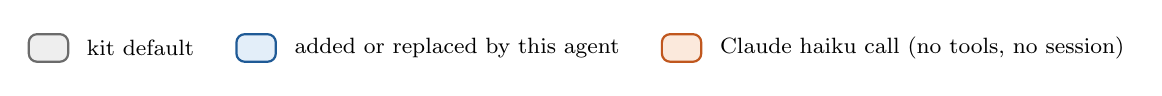
\begin{tikzpicture}[baseline=-0.6ex]
  \node[kitbox, minimum height=0.35cm, minimum width=0.5cm] (k) {};
  \node[right=1mm of k, font=\footnotesize] (kt) {kit default};
  \node[ownbox, minimum height=0.35cm, minimum width=0.5cm, right=4mm of kt] (o) {};
  \node[right=1mm of o, font=\footnotesize] (ot) {added or replaced by this agent};
  \node[llmbox, minimum height=0.35cm, minimum width=0.5cm, right=4mm of ot] (l) {};
  \node[right=1mm of l, font=\footnotesize] {Claude haiku call (no tools, no session)};
\end{tikzpicture}

\vspace{2mm}
\noindent{\bfseries Fig.~1} Processes and data flow\par
\vspace{1mm}
\begin{center}
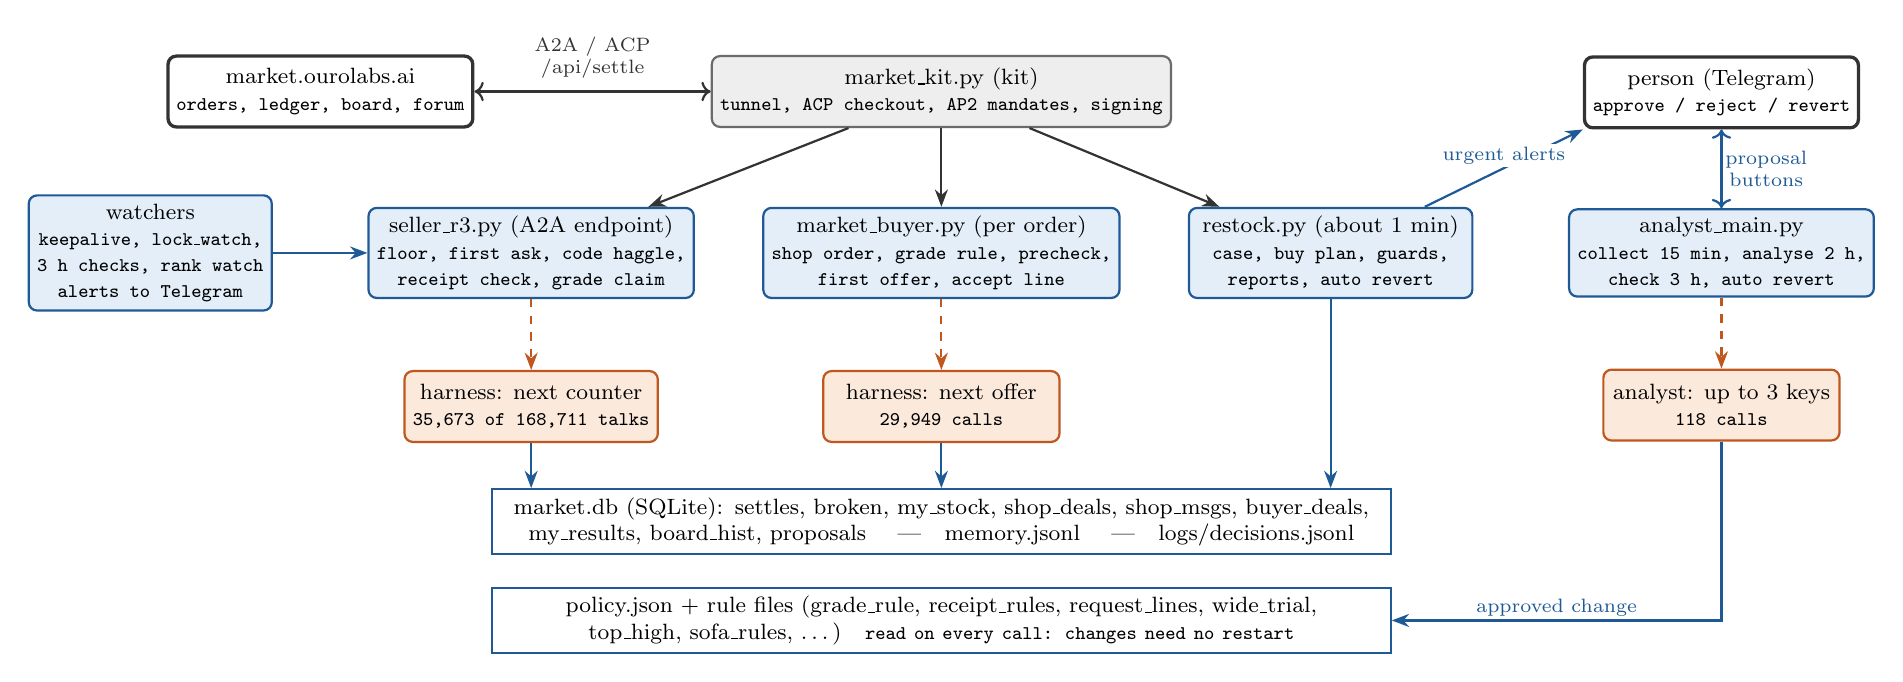
\begin{tikzpicture}[node distance=6mm and 9mm]
  % market and kit
  \node[extbox, minimum width=3.2cm] (market) {market.ourolabs.ai\\ \fn{orders, ledger, board, forum}};
  \node[kitbox, right=30mm of market, minimum width=4.6cm] (kit)
       {market\_kit.py (kit)\\ \fn{tunnel, ACP checkout, AP2 mandates, signing}};
  \draw[a, <->] (market) -- node[font=\scriptsize, align=center, above=1pt]{A2A / ACP\\ /api/settle} (kit);

  % three hooks the kit starts
  \node[ownbox, below left=10mm and 2mm of kit, minimum width=3.6cm] (seller)
       {seller\_r3.py (A2A endpoint)\\ \fn{floor, first ask, code haggle,}\\ \fn{receipt check, grade claim}};
  \node[ownbox, below=10mm of kit, minimum width=3.6cm] (buyer)
       {market\_buyer.py (per order)\\ \fn{shop order, grade rule, precheck,}\\ \fn{first offer, accept line}};
  \node[ownbox, below right=10mm and 2mm of kit, minimum width=3.6cm] (restock)
       {restock.py (about 1 min)\\ \fn{case, buy plan, guards,}\\ \fn{reports, auto revert}};
  \draw[a] (kit) -- (seller);
  \draw[a] (kit) -- (buyer);
  \draw[a] (kit) -- (restock);

  % harness
  \node[llmbox, below=9mm of seller, minimum width=3.0cm] (h1) {harness: next counter\\ \fn{35,673 of 168,711 talks}};
  \node[llmbox, below=9mm of buyer, minimum width=3.0cm] (h2) {harness: next offer\\ \fn{29,949 calls}};
  \draw[al] (seller) -- (h1);
  \draw[al] (buyer) -- (h2);

  % memory
  \node[store, below=24mm of buyer] (db)
       {market.db (SQLite): settles, broken, my\_stock, shop\_deals, shop\_msgs, buyer\_deals, my\_results, board\_hist, proposals
        \quad|\quad memory.jsonl \quad|\quad logs/decisions.jsonl};
  \node[store, below=4mm of db] (pol)
       {policy.json + rule files (grade\_rule, receipt\_rules, request\_lines, wide\_trial, top\_high, sofa\_rules, \dots)\quad
        \fn{read on every call: changes need no restart}};
  \draw[ao] (h1.south) -- (h1.south |- db.north);
  \draw[ao] (h2.south) -- (h2.south |- db.north);
  \draw[ao] (restock.south) -- (restock.south |- db.north);

  % analyst, person, watchers
  \node[ownbox, right=12mm of restock, minimum width=3.4cm] (analyst)
       {analyst\_main.py\\ \fn{collect 15 min, analyse 2 h,}\\ \fn{check 3 h, auto revert}};
  \node[llmbox, below=9mm of analyst, minimum width=3.0cm] (h3) {analyst: up to 3 keys\\ \fn{118 calls}};
  \draw[al] (analyst) -- (h3);
  \node[extbox, above=10mm of analyst, minimum width=3.4cm] (person) {person (Telegram)\\ \fn{approve / reject / revert}};
  \draw[ao, <->] (analyst) -- node[lab, right]{proposal\\ buttons} (person);
  \draw[ao] (restock) -- node[lab, above]{urgent alerts} (person.south west);
  \node[ownbox, left=12mm of seller, minimum width=3.0cm] (watch)
       {watchers\\ \fn{keepalive, lock\_watch,}\\ \fn{3 h checks, rank watch}\\ \fn{alerts to Telegram}};
  \draw[ao] (watch) -- (seller);
  \draw[ao] (h3.south) |- node[lab, pos=0.75, above]{approved change} (pol.east);
\end{tikzpicture}
\end{center}

\vspace{1mm}
\noindent{\bfseries Fig.~2} Decision order inside one negotiation (code decides; the harness only picks some next moves)\par
\vspace{1mm}
\begin{center}
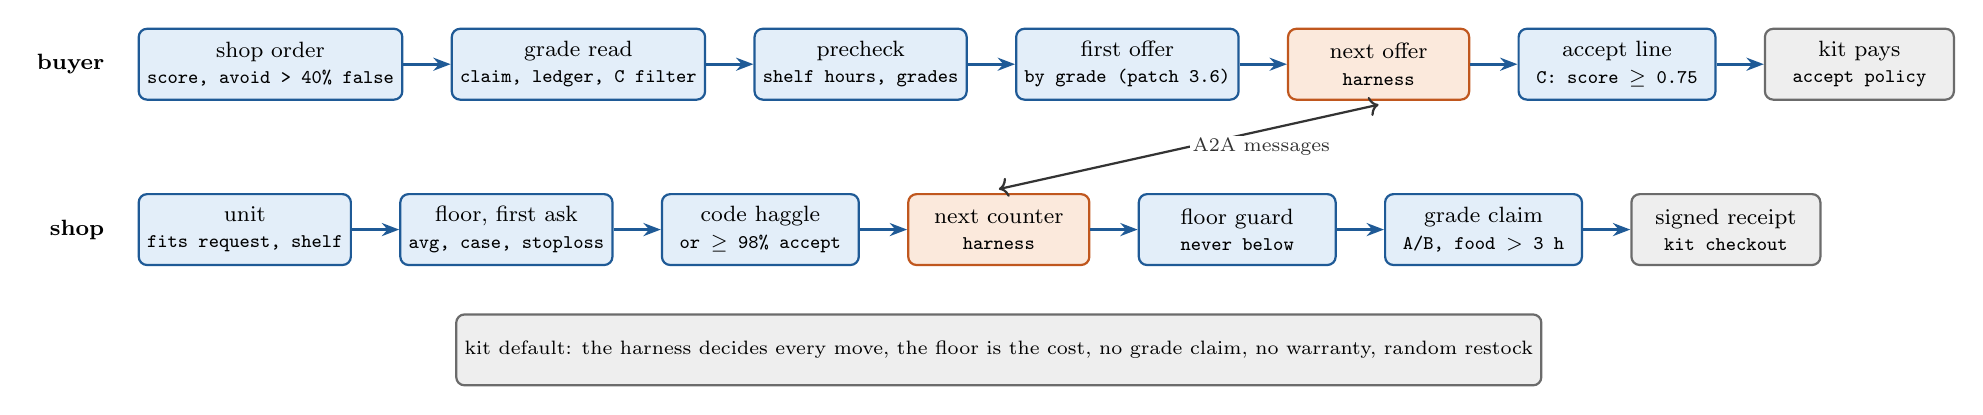
\begin{tikzpicture}[node distance=5mm and 6mm]
  % buyer row
  \node[font=\footnotesize\bfseries, anchor=east] (bl) at (0,0) {buyer};
  \node[ownbox, right=3mm of bl, minimum width=2.5cm] (b1) {shop order\\ \fn{score, avoid > 40\% false}};
  \node[ownbox, right=of b1, minimum width=2.5cm] (b2) {grade read\\ \fn{claim, ledger, C filter}};
  \node[ownbox, right=of b2, minimum width=2.5cm] (b3) {precheck\\ \fn{shelf hours, grades}};
  \node[ownbox, right=of b3, minimum width=2.5cm] (b4) {first offer\\ \fn{by grade (patch 3.6)}};
  \node[llmbox, right=of b4, minimum width=2.3cm] (b5) {next offer\\ \fn{harness}};
  \node[ownbox, right=of b5, minimum width=2.5cm] (b6) {accept line\\ \fn{C: score $\ge$ 0.75}};
  \node[kitbox, right=of b6, minimum width=2.4cm] (b7) {kit pays\\ \fn{accept policy}};
  \foreach \x/\y in {b1/b2,b2/b3,b3/b4,b4/b5,b5/b6,b6/b7} \draw[flow, own] (\x) -- (\y);

  % seller row
  \node[font=\footnotesize\bfseries, anchor=east] (sl) at (0,-2.1) {shop};
  \node[ownbox, right=3mm of sl, minimum width=2.5cm] (s1) {unit\\ \fn{fits request, shelf}};
  \node[ownbox, right=of s1, minimum width=2.5cm] (s2) {floor, first ask\\ \fn{avg, case, stoploss}};
  \node[ownbox, right=of s2, minimum width=2.5cm] (s3) {code haggle\\ \fn{or $\ge$ 98\% accept}};
  \node[llmbox, right=of s3, minimum width=2.3cm] (s4) {next counter\\ \fn{harness}};
  \node[ownbox, right=of s4, minimum width=2.5cm] (s5) {floor guard\\ \fn{never below}};
  \node[ownbox, right=of s5, minimum width=2.5cm] (s6) {grade claim\\ \fn{A/B, food $>$ 3 h}};
  \node[kitbox, right=of s6, minimum width=2.4cm] (s7) {signed receipt\\ \fn{kit checkout}};
  \foreach \x/\y in {s1/s2,s2/s3,s3/s4,s4/s5,s5/s6,s6/s7} \draw[flow, own] (\x) -- (\y);

  \draw[a, <->] ($(b5.south)+(0,-0.05)$) -- node[lab, right]{A2A messages} ($(s4.north)+(0,0.05)$);
  \node[kitbox, below=6mm of s4, minimum width=9cm, font=\scriptsize] (kd)
       {kit default: the harness decides every move, the floor is the cost, no grade claim, no warranty, random restock};
\end{tikzpicture}
\end{center}

% ---------------------------------------------------------------- Fig. 3: roles and decision flow
% Sources (11/18): depts/dept_reports.py, depts/ceo.py, depts/ceo_policy.py, depts/qc.py, analyst_main.py,
% depts/analyst_brain.py, depts/analyst.py, depts/policy_notify.py, depts/analyst_apply.py, depts/auto_reject.py, policy.py
\newpage
\noindent{\bfseries Fig.~3} Roles and decision flow (who may change policy, and who wins)\par
\vspace{2mm}
\begin{center}
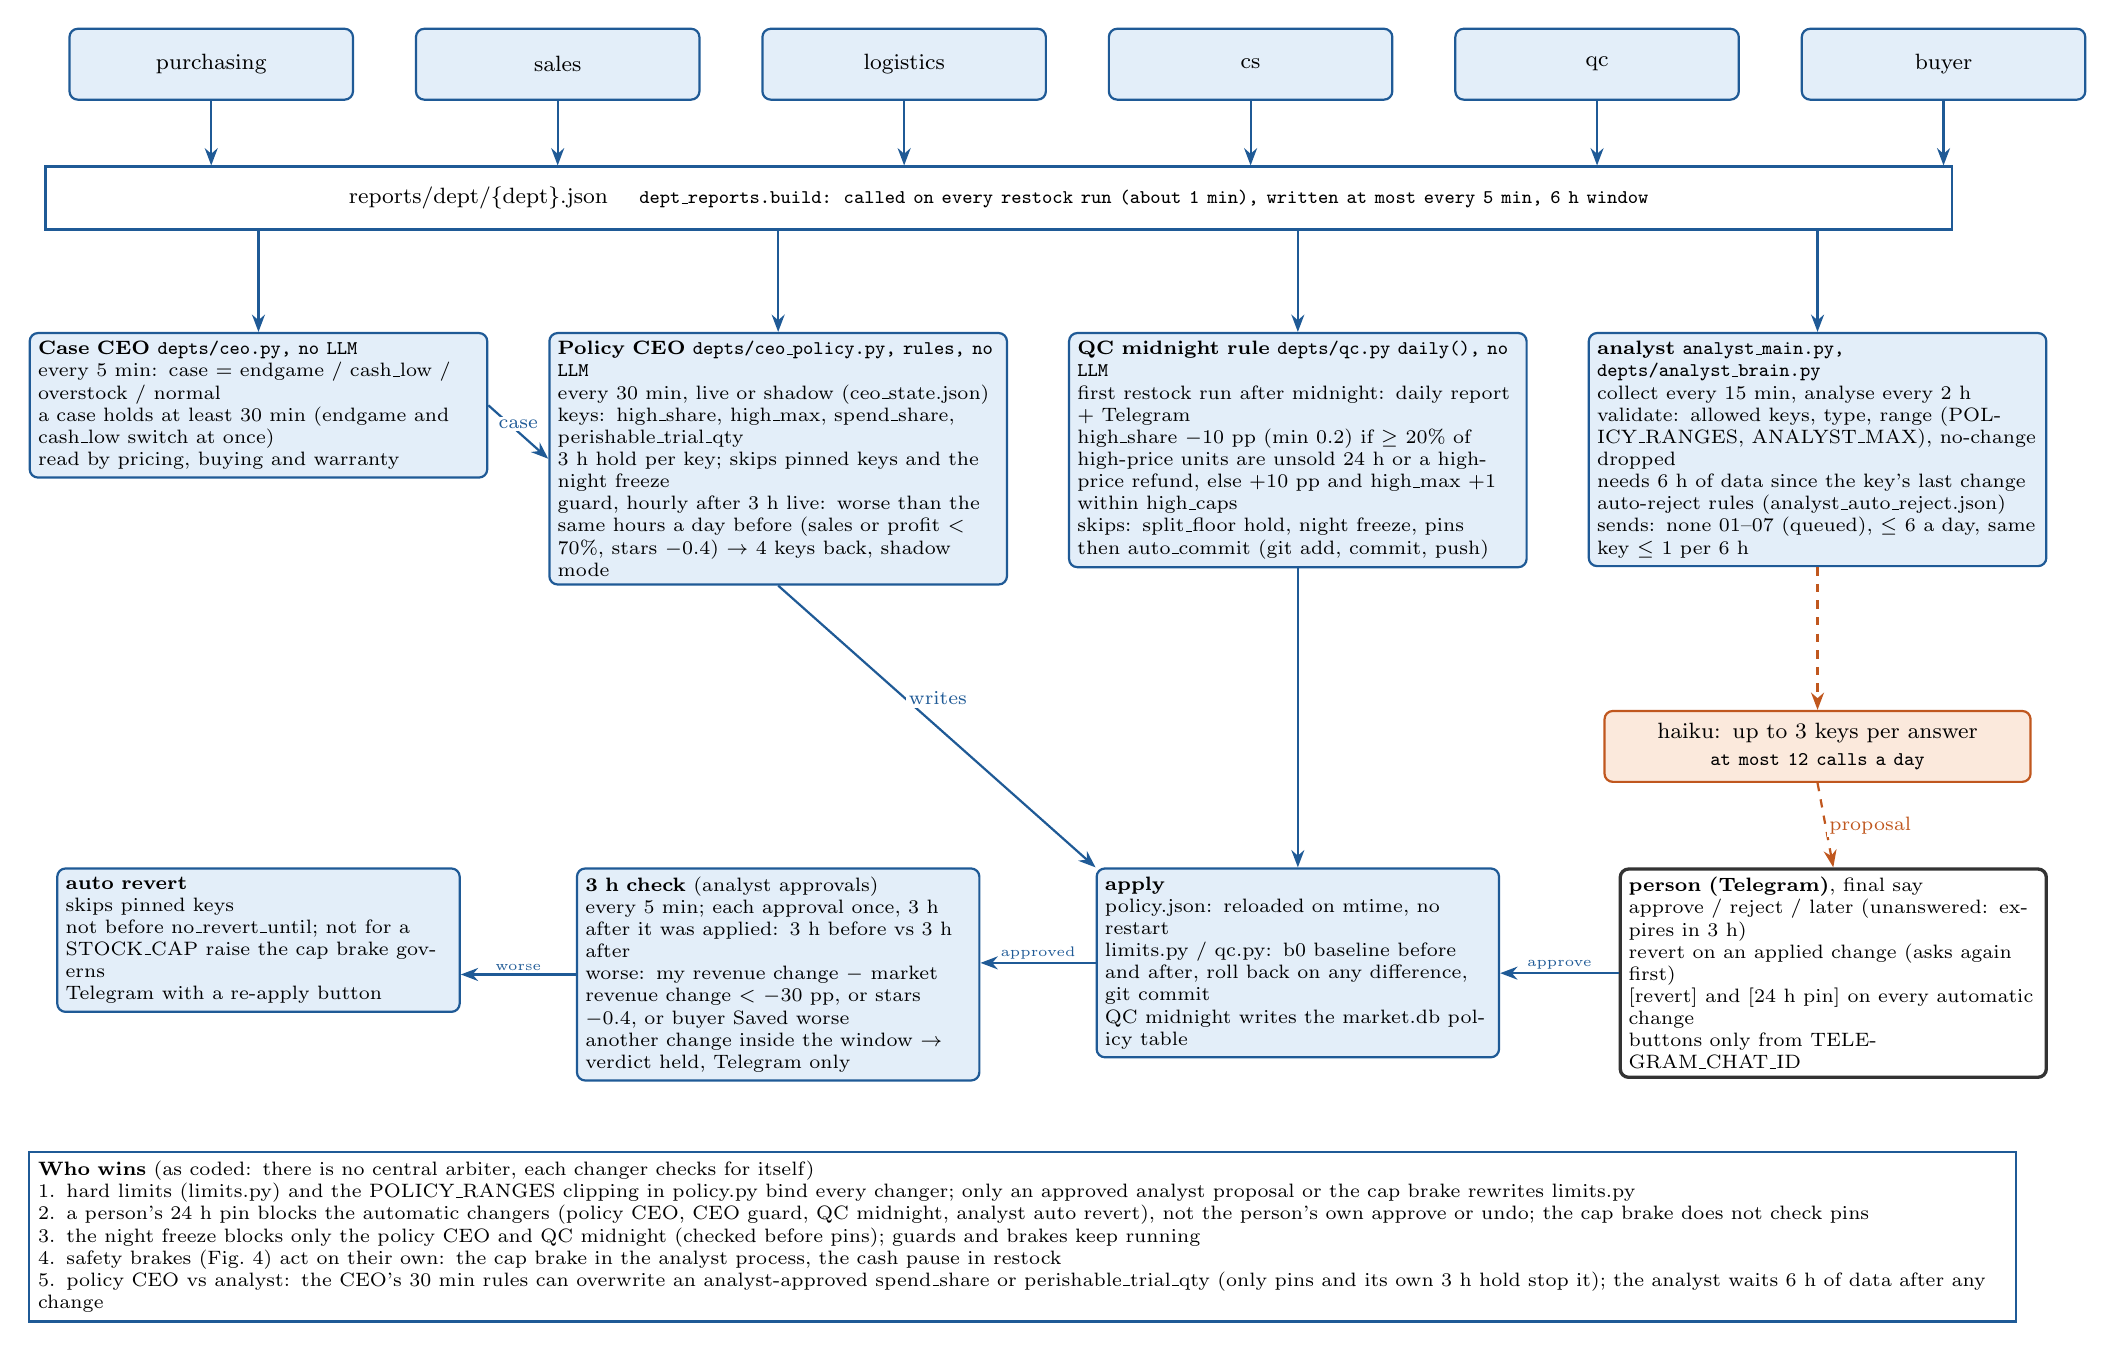
\begin{tikzpicture}[x=1cm, y=1cm]
  \tikzset{role/.style={ownbox, anchor=north, text width=5.6cm, align=left, font=\scriptsize}}
  % six departments
  \foreach \dn [count=\i] in {purchasing, sales, logistics, cs, qc, buyer}
    \node[ownbox, minimum width=3.6cm] (d\i) at ({-1.8+4.4*\i}, 0) {\dn};
  \node[store, text width=24cm] (rep) at (12.6,-1.7)
       {reports/dept/\{dept\}.json \quad \fn{dept\_reports.build: called on every restock run (about 1 min),
        written at most every 5 min, 6 h window}};
  \foreach \i in {1,...,6} \draw[ao] (d\i.south) -- (d\i.south |- rep.north);

  % the four changers
  \node[role] (case) at (3.2,-3.4) {\textbf{Case CEO} \fn{depts/ceo.py, no LLM}\\
       every 5 min: case = endgame / cash\_low / overstock / normal\\
       a case holds at least 30 min (endgame and cash\_low switch at once)\\
       read by pricing, buying and warranty};
  \node[role] (pceo) at (9.8,-3.4) {\textbf{Policy CEO} \fn{depts/ceo\_policy.py, rules, no LLM}\\
       every 30 min, live or shadow (ceo\_state.json)\\
       keys: high\_share, high\_max, spend\_share, perishable\_trial\_qty\\
       3 h hold per key; skips pinned keys and the night freeze\\
       guard, hourly after 3 h live: worse than the same hours a day before
       (sales or profit $<$ 70\%, stars $-$0.4) $\rightarrow$ 4 keys back, shadow mode};
  \node[role] (qc) at (16.4,-3.4) {\textbf{QC midnight rule} \fn{depts/qc.py daily(), no LLM}\\
       first restock run after midnight: daily report + Telegram\\
       high\_share $-$10 pp (min 0.2) if $\ge$ 20\% of high-price units are unsold 24 h or a high-price refund,
       else +10 pp and high\_max +1 within high\_caps\\
       skips: split\_floor hold, night freeze, pins\\
       then auto\_commit (git add, commit, push)};
  \node[role] (an) at (23.0,-3.4) {\textbf{analyst} \fn{analyst\_main.py, depts/analyst\_brain.py}\\
       collect every 15 min, analyse every 2 h\\
       validate: allowed keys, type, range (POLICY\_RANGES, ANALYST\_MAX), no-change dropped\\
       needs 6 h of data since the key's last change\\
       auto-reject rules (analyst\_auto\_reject.json)\\
       sends: none 01--07 (queued), $\le$ 6 a day, same key $\le$ 1 per 6 h};
  \foreach \n in {case, pceo, qc, an} \draw[ao] (rep.south -| \n.north) -- (\n.north);
  \draw[ao] (case.east) -- node[lab, above]{case} (pceo.west);

  \node[llmbox, anchor=north, text width=5.2cm] (hk) at (23.0,-8.2) {haiku: up to 3 keys per answer\\ \fn{at most 12 calls a day}};
  \draw[al] (an.south) -- (hk.north);

  % person, apply, check, revert
  \node[extbox, anchor=north, text width=5.2cm, align=left, font=\scriptsize] (person) at (23.2,-10.2)
       {\textbf{person (Telegram)}, final say\\
        approve / reject / later (unanswered: expires in 3 h)\\
        revert on an applied change (asks again first)\\
        {[}revert{]} and {[}24 h pin{]} on every automatic change\\
        buttons only from TELEGRAM\_CHAT\_ID};
  \draw[al] (hk.south) -- node[lab, right]{proposal} (person.north);
  \node[role, text width=4.9cm] (apply) at (16.4,-10.2) {\textbf{apply}\\
       policy.json: reloaded on mtime, no restart\\
       limits.py / qc.py: b0 baseline before and after, roll back on any difference, git commit\\
       QC midnight writes the market.db policy table};
  \draw[ao] (person.west) -- node[lab, above, font=\tiny]{approve} (person.west -| apply.east);
  \draw[ao] (pceo.south) -- node[lab, right, pos=0.4]{writes} (apply.north west);
  \draw[ao] (qc.south) -- (apply.north);
  \node[role, text width=4.9cm] (check) at (9.8,-10.2) {\textbf{3 h check} (analyst approvals)\\
       every 5 min; each approval once, 3 h after it was applied: 3 h before vs 3 h after\\
       worse: my revenue change $-$ market revenue change $<$ $-$30 pp, or stars $-$0.4, or buyer Saved worse\\
       another change inside the window $\rightarrow$ verdict held, Telegram only};
  \draw[ao] (apply.west) -- node[lab, above, font=\tiny, align=center]{approved} (apply.west -| check.east);
  \node[role, text width=4.9cm] (rev) at (3.2,-10.2) {\textbf{auto revert}\\
       skips pinned keys\\
       not before no\_revert\_until; not for a STOCK\_CAP raise the cap brake governs\\
       Telegram with a re-apply button};
  \draw[ao] (check.west) -- node[lab, above, font=\tiny]{worse} (check.west -| rev.east);

  % priority
  \node[draw=own, thick, fill=white, anchor=north, text width=25cm, align=left, font=\scriptsize] at (12.9,-13.8)
       {\textbf{Who wins} (as coded: there is no central arbiter, each changer checks for itself)\\
        1. hard limits (limits.py) and the POLICY\_RANGES clipping in policy.py bind every changer;
           only an approved analyst proposal or the cap brake rewrites limits.py\\
        2. a person's 24 h pin blocks the automatic changers (policy CEO, CEO guard, QC midnight, analyst auto revert),
           not the person's own approve or undo; the cap brake does not check pins\\
        3. the night freeze blocks only the policy CEO and QC midnight (checked before pins); guards and brakes keep running\\
        4. safety brakes (Fig.~4) act on their own: the cap brake in the analyst process, the cash pause in restock\\
        5. policy CEO vs analyst: the CEO's 30 min rules can overwrite an analyst-approved spend\_share or
           perishable\_trial\_qty (only pins and its own 3 h hold stop it); the analyst waits 6 h of data after any change};
\end{tikzpicture}
\end{center}

% ---------------------------------------------------------------- Fig. 4: safety brakes and auto-reverts
% Sources (11/18): depts/wide_trial.py, limits.py, depts/cap_brake.py, cap_brake.json, tools/high_focus_rollout.py,
% depts/request_six.py, depts/request_buy.py, alerts.py, depts/supply_window.py, end_rules.json, depts/claim_full.py,
% seller_r3.py, harness.py, depts/analyst_brain.py, depts/saved_guard.py, tools/subst_always.py,
% tools/shop_order_check.py, depts/shop_avoid.py, depts/buyer_biz.py, tools/watchdog.py, keepalive.py,
% tools/stall_watch.py, tools/lock_watch.py, logs/alerts.jsonl; states as of the close (11/17 23:59)
\newcommand{\brk}[7]{\node[ownbox, anchor=north, text width=6.3cm, align=left, font=\scriptsize] at (#1,#2)
  {\textbf{#3}\\ \textbf{if} #4\\ \textbf{then} #5\\ \textbf{alert} #6\\ \textbf{state} #7};}
\newpage
\noindent{\bfseries Fig.~4} Safety brakes and auto-reverts (condition $\rightarrow$ action $\rightarrow$ alert), 1/2: stock, cash, selling\par
\vspace{2mm}
\begin{center}
\begin{tikzpicture}[x=1cm, y=1cm]
  \brk{3.4}{0}{60M high-cost brake \fn{depts/wide\_trial.py}}
      {cost of high-price units unsold 12 h+ $>$ 60,000,000}
      {trial B, C, TWO off; high\_max 100}{urgent}
      {fired 11/13 21:08 (148 units, 60,090,456); on again by the person 11/14 about 16:10}
  \brk{10.2}{0}{Automatic re-on \fn{wide\_trial.re\_on}}
      {after a trip, that cost stays $<$ 45,000,000 for 6 h (the clock resets after a 30 min gap)}
      {trial on, high\_max 120}{urgent}{never fired}
  \brk{17.0}{0}{Automatic STOCK\_CAP \fn{limits.py}}
      {every restock run}
      {cap = cash + stock $-$ 5,000,000 reserve}{none}{ended at the 11/17 17:59 end cap}
  \brk{23.8}{0}{STOCK\_CAP brake \fn{depts/cap\_brake.py}}
      {every 5 min, 2 hits in a row: sale median $>$ 4 h over 6 h ($\ge$ 10 sales), or unsold $>$ 35\% and
       $>$ 5M of units 12 h+ old, or cash $<$ 4M}
      {STOCK\_CAP 20,000,000, automatic cap off, git commit}{urgent; info before the 2nd hit}
      {stock trips warn only since 11/10 (person); the cash trip still acts}
  \brk{3.4}{-4.2}{Cash pause \fn{cap\_brake, limits.buy\_paused}}
      {automatic cap on and cash $<$ 4,000,000}
      {restock buys nothing until cash $>$ 5,000,000}{urgent (pause), info (resume)}{in code}
  \brk{10.2}{-4.2}{Cash floor \fn{depts/ceo.py}}
      {cash $<$ 1,000,000}
      {case cash\_low, no restock}{log line only, no Telegram}{in code}
  \brk{17.0}{-4.2}{High-price brake \fn{tools/high\_focus\_rollout.py}}
      {every 15 min, 2 hits: sale median over 6 h, or 12 h+ unsold $>$ 30\% ($\ge$ 10 units), or receipt
       ratio $\le$ 1/3 of base}
      {would set high\_max 60, high\_share 0.7}{info, hourly}
      {warn only since 11/10; warned many times 11/13--11/15}
  \brk{23.8}{-4.2}{Normal-stock revert \fn{depts/request\_six.py}}
      {normal stock unsold 12 h+ costs $>$ 10,000,000}
      {request lines 6 $\rightarrow$ 4 (3 regular + 1 trial)}{urgent}{never fired}
  \brk{3.4}{-8.4}{Trial request lines \fn{depts/request\_buy.py}}
      {6 h after the first trial buy the sale median is not $\le$ 1 h, or no sale in 24 h}
      {SKU dropped from the candidates}{decision log only}{in code}
  \brk{10.2}{-8.4}{Volume-pricing guard \fn{alerts.volume\_guard}}
      {6 h profit $<$ 70\% of the 6 h before}
      {volume pricing reverted}{urgent}{in code}
  \brk{17.0}{-8.4}{Supply-window guard \fn{depts/supply\_window.py}}
      {more than 6 lines refused as closed in 3 h}
      {back to 12 s per line}{Telegram}{fired at 11 s; 11.5 s at the close}
  \brk{23.8}{-8.4}{End of round \fn{end\_rules.json, limits.py}}
      {11/17 17:59 (6 h before the close); endgame pricing in the last 12 h}
      {restock stops; STOCK\_CAP 15,000,000, automatic cap off; price cost $-$10\% per 6 h, floor = cost;
       food bought only if it lasts past the close}
      {urgent (cap\_end)}{ran 11/17 17:59 (commit 05bbff3)}
  \brk{3.4}{-12.6}{Sofa warranty off \fn{alerts.sofa\_warranty\_check}}
      {48 h sofa refunds $>$ 30\% of 48 h sofa profit}
      {sofa\_rules.json warranty false}{urgent}{fired 11/10 and 11/13; off at the close}
  \brk{10.2}{-12.6}{Grade-claim guard \fn{depts/claim\_full.py}}
      {any false claim since the switch}
      {non-food claim\_share back to 0.5; a false food claim turns food claims off (non-food kept)}{urgent}
      {never fired: 5,747 claims, all honest (board 11/17 23:59)}
  \brk{17.0}{-12.6}{Seller floor guard \fn{seller\_r3.py}}
      {the harness accepts or asks below the floor}
      {code counter instead}{none}{in code}
  \brk{23.8}{-12.6}{Negotiation expiry \fn{depts/open\_expiry.py}}
      {a negotiation quiet for 5 min}
      {closed, unit freed}{none}{open\_expiry.json 300 s since 11/09}
\end{tikzpicture}
\end{center}

\newpage
\noindent{\bfseries Fig.~4} Safety brakes and auto-reverts (condition $\rightarrow$ action $\rightarrow$ alert), 2/2: buyer, LLM, processes, checks\par
\vspace{2mm}
\begin{center}

\begin{tikzpicture}[x=1cm, y=1cm]
  \brk{3.4}{0}{Saved guard \fn{depts/saved\_guard.py}}
      {my Saved $<$ the student just below + 0.008}
      {grade A deals use the B/C moves (0.65 / 1.00); back at + 0.015}{urgent}
      {fired 11/13 07:46; switch locked by the person 11/13 about 13:20}
  \brk{10.2}{0}{Min-offers guard \fn{alerts.buyer\_mo\_guard}}
      {Saved rank worse than at the min-offers change, 2 board snapshots in a row}
      {weights back to 0.8 / 0.2, once}{urgent}{in code}
  \brk{17.0}{0}{Substitute plan A stop \fn{tools/subst\_always.py}}
      {$\ge$ 20 A receipts in 24 h and: paid $<$ 30\%, or mismatch reviews $\ge$ 5 and $\ge$ 10\%, or stars
       $\le$ normal $-$ 0.3 (checked every 30 min)}
      {mode B: ``not in stock'' at once}{urgent}{stopped 11/14 02:10 (paid 23/80)}
  \brk{23.8}{0}{Shop-order guard \fn{tools/shop\_order\_check.py}}
      {$\ge$ 100 orders in 2 h and close rate $<$ base $-$ 5 pp, or deals per hour $<$ 80\% of base}
      {stock\_first and rate\_order off}{urgent}{stopped (30.0 $<$ 39.3 $\times$ 80\%)}
  \brk{3.4}{-4.2}{Shop-avoid warning \fn{depts/shop\_avoid.py}}
      {$\ge$ 5 orders missed by the avoid rules in 2 h}
      {rules stay on; a warning at most every 2 h}{urgent}{fired 3 times}
  \brk{10.2}{-4.2}{Receipt refused \fn{buyer\_biz.refuse\_receipt}}
      {receipt amount, item or budget does not match the deal}
      {receipt not handed to the kit: no payment}{urgent}{in code}
  \brk{17.0}{-4.2}{LLM failure, seller and buyer \fn{seller\_r3.py, harness.py}}
      {a harness call fails}
      {seller: code haggle (next counter, accept at or above it); buyer: soft\_neg or code moves}
      {info per failure; urgent after more than 10 in a row}{in code}
  \brk{23.8}{-4.2}{Analyst LLM pause \fn{depts/analyst\_brain.py}}
      {usage-limit text in the answer}
      {pause until the named reset, else 1 h; at most 12 calls a day}{urgent}{in code}
  \brk{3.4}{-8.4}{watchdog \fn{tools/watchdog.py}}
      {every 60 s: analyst missing; seller missing 2 checks or no buyer line for 600 s; keepalive missing}
      {restart (the kit tree is killed, keepalive starts it again); more than 3 restarts in 1 h for one
       name $\rightarrow$ no restart of it for 1 h}
      {urgent (restart, stop, kit flapping)}{stopped 11/18 12:07}
  \brk{10.2}{-8.4}{keepalive \fn{keepalive.py}}
      {3 missed agent-card checks, 60 s apart}
      {kit restart}{none}{stopped 11/18 12:07}
  \brk{17.0}{-8.4}{stall\_watch \fn{tools/stall\_watch.py}}
      {every 5 min: no sale in 30 min, no order in 10 min, or cash $\ge$ 5M with 2 empty supply windows}
      {one kit restart; still stalled 15 min later $\rightarrow$ 2nd alert; board offline 2 reads $\rightarrow$ alert only}
      {urgent}{stopped 11/18 12:07}
  \brk{23.8}{-8.4}{lock\_watch \fn{tools/lock\_watch.py}}
      {locked share $>$ 20\%}
      {none (measure only)}{urgent}{in code}
  \brk{3.4}{-12.6}{Analyst 3 h check \fn{depts/analyst\_apply.py}}
      {3 h after an approval: worse than the 3 h before, market-adjusted (Fig.~3)}
      {auto revert (pins kept); verdict held if another change is in the window}
      {Telegram with a re-apply button}{in code}
  \brk{10.2}{-12.6}{Policy CEO guard \fn{depts/ceo\_policy.py}}
      {hourly after 3 h live: sales or profit $<$ 70\% of the same hours a day before, or stars $-$0.4}
      {4 CEO keys back (pins kept), shadow mode}{Telegram}{in code}
\end{tikzpicture}
\end{center}

% ---------------------------------------------------------------- Korean notes
\newpage
\setlist{nosep, leftmargin=1.2em}
\hangulfont\kpage{Architecture notes}{그림 1--4 한글 설명}
\small\linespread{1.25}\selectfont\setlength{\parskip}{3pt}
\setlength{\columnsep}{9mm}\setlength{\columnseprule}{0.4pt}\def\columnseprulecolor{\color{ownfill}}
\begin{multicols}{2}
\begin{kbox}[title=한눈에 보기]
에이전트는 키트(market\_kit.py)가 띄우는 세 명령 seller\_r3.py, market\_buyer.py, restock.py와, 따로 도는
analyst\_main.py, 감시 프로세스들로 이루어진다. 판단은 대부분 코드가 하고, 모델(Claude haiku)은 흥정의 다음 수와
분석관의 정책 제안에만 쓴다. 모델은 도구도 세션도 없이 코드가 만든 프롬프트 하나에 JSON 한 줄로 답한다.

\noindent{\bfseries 색.} 회색은 키트 기본형에 이미 있는 부분, 파란색은 우리가 만들거나 바꾼 부분, 주황색 점선은
haiku 호출이다.
\end{kbox}

\ksec{그림 1: 프로세스와 데이터 흐름}
\begin{itemize}
  \item \kname{market.ourolabs.ai}: 주문, 원장, 보드, 포럼이 있는 시장 서버.
  \item \kname{market\_kit.py (키트, 수정하지 않음)}: 터널, ACP 결제, AP2 위임, 서명을 맡고 아래 세 명령을
        띄운다. 시장과는 A2A/ACP 메시지와 /api/settle로 통신한다.
  \item \kname{seller\_r3.py}: 가게의 A2A 서버. 하한과 첫 호가를 계산하고, 코드로 흥정하고, 영수증 금액을
        합의가와 맞추고, 등급 주장을 넣는다.
  \item \kname{market\_buyer.py}: 주문마다 새로 뜨는 구매자. 가게 순서, 등급 판정, 사전 점검, 첫 제안,
        수락선을 정한다.
  \item \kname{restock.py}: 약 1분마다 새로 뜨는 매입과 운영 루프. 상황 판정, 매입 계획, 안전장치, 보고,
        자동 원복을 한다.
  \item \kname{harness (주황)}: 가게와 구매자가 다음 수를 정할 때만 부르는 haiku. 가게는 협상 168,711건 중
        35,673건에서, 구매자는 29,949회 불렀다(11/17 14:44 기준).
  \item \kname{market.db, memory.jsonl, decisions.jsonl}: 정산, 고장, 재고, 협상, 구매 결과, 보드 기록.
        재시작해도 남고 다음 결정(가게 순서, 매입, 가격)의 입력이 된다.
  \item \kname{policy.json과 규칙 파일}: 호출마다 다시 읽으므로 값을 바꿔도 재시작이 필요 없다.
  \item \kname{analyst\_main.py}: 15분마다 수집하고 2시간마다 분석해 정책 키를 한 번에 최대 3개 제안한다(haiku
        118회, 하루 12회 한도). 분석 주기는 11/06 저녁에 1시간에서 2시간으로 바뀌었다(analyst\_brain.py ANALYSE\_S).
  \item \kname{person (Telegram)}: 분석관 제안을 승인, 거절, 원복하고 restock의 긴급 알림을 받는다. 승인된
        변경만 정책 파일에 들어가고, 3시간 뒤 비교에서 나빠지면 자동으로 원복된다.
  \item \kname{watchers}: keepalive, lock\_watch, 3시간 점검, 순위 감시. 이상이 있으면 텔레그램으로 알린다.
\end{itemize}

\columnbreak
\ksec{그림 2: 한 협상 안의 결정 순서}
코드가 순서대로 결정하고, 하네스는 중간의 다음 수 하나만 고른다. 가게 협상의 약 73\%는 하네스 없이 코드
흥정으로 끝난다. 두 줄은 A2A 메시지로 이어진다.

\ksub{구매자 (buyer)}
\begin{enumerate}
  \item 가게 순서: 지난 24시간 가게 점수 순. 거짓 등급 주장이 40\%를 넘는 가게는 피한다.
  \item 등급 판정: 가게의 주장과 원장 기록으로 등급을 읽고 C를 거른다.
  \item 사전 점검: 결제 정책(남은 유통기한, 받을 등급)에 걸릴 유닛은 흥정 전에 거른다.
  \item 첫 제안: 등급별 비율로 계산한다(patch 3.6의 Saved 점수식).
  \item 다음 제안: 하네스.
  \item 수락선: C는 기대 점수 0.75 이상일 때만 받는다.
  \item 결제: 키트가 결제 정책을 확인한 뒤 지불한다.
\end{enumerate}

\ksub{가게 (shop)}
\begin{enumerate}
  \item 유닛: 요청과 남은 유통기한에 맞는 유닛을 고른다.
  \item 하한과 첫 호가: 시장 평균, 상황(case), 손절 규칙으로 정한다.
  \item 코드 흥정: 직전 호가의 98\% 이상이면 바로 수락한다.
  \item 다음 호가: 하네스.
  \item 하한 가드: 하네스가 무엇을 말해도 하한 아래로는 내려가지 않는다.
  \item 등급 주장: A와 B만. 식품은 다음 등급 하락까지 3시간 넘게 남은 유닛만.
  \item 서명된 영수증: 키트 checkout으로 정산된다.
\end{enumerate}

\ksec{키트 기본형과 다른 점}
\begin{enumerate}
  \item 결정의 주체: 기본형은 하네스가 모든 수를 정한다. 우리는 코드가 대부분 정하고 하네스는 흥정의 일부만 맡는다.
  \item 기억의 위치: 기본형은 기억이 없다. 우리는 market.db와 요약 파일이 다음 결정의 입력이 된다.
  \item 사람과 안전장치: 기본형에는 운영 루프가 없다. 우리는 분석관 제안, 사람 승인, 반영, 자동 비교와 원복으로
        이어지는 고리가 있다.
  \item 그 밖에 기본형은 하한이 원가이고, 등급 주장과 보증이 없고, 재고를 무작위로 채운다.
\end{enumerate}
\end{multicols}

% ---------------------------------------------------------------- Korean notes: Fig. 3, Fig. 4
\newpage
\hangulfont\small\linespread{1.25}\selectfont\setlength{\parskip}{3pt}
\kpage{Roles and safety}{그림 3, 4 한글 설명}
\ksec{그림 3: 역할 분담과 결정 흐름}
\begin{itemize}
  \item 부서 6개(purchasing, sales, logistics, cs, qc, buyer)의 보고서는 dept\_reports.build가 만든다. restock이 돌 때마다
        부르지만 5분에 한 번만 쓰고, 최근 6시간을 본다(reports/dept/*.json).
  \item 정책을 바꿀 수 있는 주체는 넷이다. 모두 코드 규칙이고, LLM은 분석관의 제안 단계에서만 쓴다.
  \begin{itemize}
    \item Case CEO(depts/ceo.py): 5분마다 상황(endgame, cash\_low, overstock, normal)을 정한다. 한 번 정하면 30분은 유지하고,
          endgame과 cash\_low는 바로 바꾼다.
    \item Policy CEO(depts/ceo\_policy.py): 30분마다 키 4개(high\_share, high\_max, spend\_share, perishable\_trial\_qty)만 바꾼다.
          키마다 3시간 유지, 사람이 고정한 키와 야간 동결은 건너뛴다. live 3시간 뒤부터 매시간 전날 같은 시간대와 비교해
          판매나 이익이 70\% 미만이거나 별점이 0.4 떨어지면 4개 키를 되돌리고 shadow로 내려간다.
    \item QC 자정 규칙(depts/qc.py daily): 자정 뒤 첫 restock에서 일일 보고서와 텔레그램을 보내고, 고가 비중과 개수를
          조정한 뒤 자동 커밋을 한다.
    \item 분석관(analyst): 15분 수집, 2시간 분석. haiku가 키를 최대 3개 제안하면 허용 키, 형식, 범위, 6시간 근거, 자동 거절
          규칙을 코드가 검사한다. 01--07시에는 보내지 않고 모아 두며, 하루 6건, 같은 키는 6시간에 한 번까지 보낸다.
  \end{itemize}
  \item 사람(텔레그램)이 최종 결정권을 가진다. 제안에는 승인, 거절, 나중에 버튼이 있고(답이 없으면 3시간 뒤 만료),
        자동 변경 알림에는 모두 되돌리기와 24시간 고정 버튼이 붙는다. 되돌리기는 한 번 더 묻는다.
  \item 승인된 변경은 policy.json(수정 시각을 보고 다시 읽음, 재시작 없음)이나 limits.py(바꾸기 전후 b0 기준 실행, 차이가
        나면 되돌리고 git 커밋)에 들어간다.
  \item 3시간 점검: 승인 3시간 뒤 한 번, 앞뒤 3시간을 비교한다. 내 매출 변화에서 시장 매출 변화를 뺀 값이 $-$30\%p보다
        나쁘거나, 별점이 0.4 떨어지거나, 구매자 Saved가 나빠지면 자동 원복한다. 비교 구간에 다른 변경이 섞이면 판정을
        보류하고 텔레그램만 보낸다.
\end{itemize}

\begin{kbox}[title=충돌 우선순위 (코드 기준)]
 한곳에서 순서를 정하는 함수는 없고, 각 주체가 스스로 확인한다.
\begin{enumerate}
  \item 하드 한도(limits.py)와 policy.py의 범위 자르기는 모두에게 적용된다. limits.py는 승인된 분석관 제안과 cap brake만 고친다.
  \item 사람의 24시간 고정은 자동 주체(Policy CEO, CEO 가드, QC 자정, 분석관 자동 원복)를 막는다. 사람 자신의 승인이나
        되돌리기는 막지 않고, cap brake는 고정을 보지 않는다.
  \item 야간 동결은 Policy CEO와 QC 자정만 막는다(고정보다 먼저 확인). 가드와 브레이크는 계속 돈다.
  \item 안전장치(그림 4)는 따로 움직인다. cap brake는 분석관 프로세스에서, 현금 정지는 restock에서 돈다.
  \item Policy CEO와 분석관: CEO의 30분 규칙은 분석관 승인으로 바뀐 spend\_share, perishable\_trial\_qty를 다시 바꿀 수 있다
        (막는 것은 고정과 CEO 자신의 3시간 유지뿐). 분석관은 어떤 변경 뒤든 6시간 근거를 기다린다.
\end{enumerate}
\end{kbox}

\ksec{그림 4: 안전장치와 자동 원복}
상자마다 조건(if), 동작(then), 알림(alert), 마감 시점 상태(state)를 적었다. state가 “in code”인 것은 코드에 있지만
마감까지 동작한 기록을 따로 세지 않은 것이다. 경고만 하도록 바꾼 장치(STOCK\_CAP 재고 조건, 고가 브레이크)는 사람이
11/10에 정했다. 숫자의 출처는 각 상자의 파일과 logs/alerts.jsonl이다.

% ---------------------------------------------------------------- Korean notes: component table
\newpage
\kpage{Components}{구성요소 전체, 11/18 코드 기준}
재시작 칸: “seller”는 seller\_r3.py 재시작, “다음 실행”은 다음 restock(약 1분, 새 프로세스), “다음 주문”은 주문마다 새로
뜨는 구매자, “없음”은 json을 호출마다 다시 읽는 것, “analyst”는 analyst\_main.py 재시작이 필요하다는 뜻이다.

{\footnotesize\color{kit}}
\footnotesize
\ksub{프로세스와 역할}
{\renewcommand{\arraystretch}{1.3}\setlength{\tabcolsep}{5pt}\rowcolors{2}{white}{ownfill!55}
\begin{xltabular}{\linewidth}{>{\raggedright\arraybackslash}p{5.2cm} Y >{\raggedright\arraybackslash}p{3.6cm} >{\raggedright\arraybackslash}p{3.2cm}}
\khead \kh{이름} & \kh{하는 일} & \kh{주기} & \kh{재시작} \\
\endhead
\kname{seller\_r3.py} & 가게 A2A 서버. 유닛 선택, 하한과 첫 호가, 코드 흥정, 영수증 & 상시, 메시지마다 & 코드: seller \\
\kname{market\_buyer.py}\kpath{depts/buyer\_biz.py} & 주문 하나를 처리하는 구매자 & 주문마다 새 프로세스 & 다음 주문 \\
\kname{restock.py} & QC 일일, 포럼(cs), 부서 보고, Policy CEO, 포럼 감시, 알림 점검, 매입 계획을 차례로 실행 & 약 1분마다 새 프로세스 & 다음 실행 \\
\kname{analyst\_main.py} & 텔레그램 폴링(25초), 분석관, 승인 3시간 점검, cap brake, 구매자 포럼 게시 스레드 & 상시 & analyst \\
\kname{harness.py} & claude -p haiku 호출(도구 없음, 세션 없음), 실패 시 코드 흥정으로 넘김 & 흥정의 다음 수마다 & 코드: seller \\
\kname{dept\_reports.build} & 부서 6개 보고서(reports/dept/*.json), 최근 6시간 & restock마다, 5분에 한 번 기록 & 다음 실행 \\
\kname{depts/ceo.py}\kpath{Case CEO} & 상황 endgame / cash\_low / overstock / normal, 최소 30분 유지 & 5분 & 다음 실행 \\
\kname{depts/ceo\_policy.py}\kpath{Policy CEO} & 키 4개 규칙 변경, LLM 없음, 가드와 shadow 전환 & 30분 & 다음 실행 \\
\kname{depts/qc.py daily} & 일일 보고서, 고가 비중과 개수 조정, 텔레그램, 자동 커밋 & 하루 1회(자정 뒤 첫 실행) & 다음 실행 \\
\kname{policy\_notify} & 자동 변경 알림마다 되돌리기, 24시간 고정 버튼(policy\_pins.json) & 변경마다 & 없음 \\
\kname{tools/watchdog.py, keepalive.py, tools/stall\_watch.py, tools/lock\_watch.py} & 프로세스 감시와 재시작, 판매와 주문 정체 감시, DB 잠금 비율 감시(그림 4) & 60초, 60초, 5분, 상시 & 각 프로세스 \\
\end{xltabular}}

\medskip
\ksub{가게: 매입}
{\renewcommand{\arraystretch}{1.3}\setlength{\tabcolsep}{5pt}\rowcolors{2}{white}{ownfill!55}
\begin{xltabular}{\linewidth}{>{\raggedright\arraybackslash}p{5.2cm} Y >{\raggedright\arraybackslash}p{3.6cm} >{\raggedright\arraybackslash}p{3.2cm}}
\khead \kh{이름} & \kh{하는 일} & \kh{주기} & \kh{재시작} \\
\endhead
\kname{요청 기반 매입}\kpath{depts/request\_buy.py, request\_six.py} & 재고가 없는데 이름으로 요청된 SKU를 매입 후보로 삼는다. request\_lines.json: 정식 3줄 + 시험 3줄.
  12시간 넘게 안 팔린 일반 재고가 1,000만을 넘으면 3+1줄로 돌아간다. 시험 SKU는 첫 매입 6시간 뒤 판매 중앙값이 1시간 이하가
  아니거나 24시간 판매가 없으면 뺀다 & 매입 계획마다 & 없음 \\
\kname{깊게 쌓기}\kpath{depts/deep\_high.py} & 24시간에 2개 이상 팔리고 중앙값 3시간 이하, 마진 10\% 이상인 고가 SKU를 2--5개(중앙값 1.5시간 이하면 7개)까지
  보유. high\_max 개수와 따로 센다 & 매입 계획마다 & 없음 \\
\kname{high\_cost\_exclude}\kpath{depts/high\_cost\_exclude.py} & 48시간 평균 원가가 시장 평균의 95\%를 넘거나(3개 이상 매입), 3개 이상 팔아 손해인 SKU는 매입 안 함 & 매입 계획마다 & 없음 \\
\kname{150만 초과 제한}\kpath{qc.HIGH\_MAX, top\_high.json} & 원가 1,500,000 초과 유닛은 top\_high 규칙에 맞는 SKU만, 보유 20개, SKU당 3개(깊게 쌓기 SKU 5개)까지 & 매입 계획마다 & HIGH\_MAX: 다음 실행, top\_high: 없음 \\
\kname{고가 매입 마진 확인}\kpath{depts/purchasing.py} & 고가 유닛은 기대 마진을 확인한 뒤 매입 & 매입 계획마다 & 다음 실행 \\
\end{xltabular}}

\medskip
\ksub{가게: 가격, 영수증, 보증}
{\renewcommand{\arraystretch}{1.3}\setlength{\tabcolsep}{5pt}\rowcolors{2}{white}{ownfill!55}
\begin{xltabular}{\linewidth}{>{\raggedright\arraybackslash}p{5.2cm} Y >{\raggedright\arraybackslash}p{3.6cm} >{\raggedright\arraybackslash}p{3.2cm}}
\khead \kh{이름} & \kh{하는 일} & \kh{주기} & \kh{재시작} \\
\endhead
\kname{하한}\kpath{depts/sales.py floor} & 손절: 원가가 시장 평균보다 (남은 일수 $\times$ 1\%) 이내로 높으면 하한 = 시장 평균(loss\_rule.json).
  aging: 24시간 뒤부터 6시간마다 $-$10\%, 손절 규칙 중에는 원가 아래로 안 감. 식품 clearance: 남은 시간 12시간 미만이면 시간당
  $-$10\%, 최대 $-$90\%. endgame: 마지막 12시간, 원가에서 6시간마다 $-$10\%, 하한 = 원가(end\_rules.json) & 협상 메시지마다 & 값: 없음, 코드: seller \\
\kname{코드 흥정}\kpath{code\_haggle.json} & 일반 유닛 100\%, 고가 유닛 30\%를 하네스 없이 흥정. 직전 호가의 98\% 이상이면 수락 & 협상마다 & 없음 \\
\kname{등급 주장}\kpath{depts/receipt\_exp.py, receipt\_rules.json} & 비식품 A, B는 claim\_share 1.0으로 주장. 식품 A, B는 다음 등급 하락까지 3시간(N=3) 넘게 남은
  유닛만. C는 주장 안 함. 등급은 영수증을 만들 때 다시 계산 & 영수증마다 & 없음 \\
\kname{영수증 금액 검증}\kpath{depts/receipt\_check.py} & 영수증 금액은 구매자 자신의 제안 문구로 정한다. 내 마지막 호가의 2배를 넘는 제안은 오타로 본다.
  하한 아래면 영수증 대신 역제안 & 수락마다 & seller \\
\kname{보증}\kpath{depts/sales.py warranty\_hours} & A 등급, normal 상황, 시장 고장률 5\% 이하(5건 이상)면 48시간. 150만 초과(top\_high)는 A, 고장 6\% 이하.
  소파 A, B 72시간(마감 때 sofa\_rules.json warranty false). TV, 냉방 B 보증(b\_warranty.json) & 협상마다 & 없음 \\
\kname{대체상품 A안}\kpath{depts/substitute.py, subst\_exp.json} & 없는 상품을 요청받으면 대체 상품을 제안. 11/14 02:10 결제율 23/80 $<$ 30\%로 중단, 이후 B안(바로 “재고 없음”) & 협상마다 & 없음 \\
\kname{협상 자동 만료}\kpath{depts/open\_expiry.py} & 5분 동안 조용한 협상을 닫고 유닛을 푼다(11/09 10분 $\rightarrow$ 5분) & 메시지마다 & 없음 \\
\end{xltabular}}

\medskip
\newpage\ksub{구매자}
{\renewcommand{\arraystretch}{1.3}\setlength{\tabcolsep}{5pt}\rowcolors{2}{white}{ownfill!55}
\begin{xltabular}{\linewidth}{>{\raggedright\arraybackslash}p{5.2cm} Y >{\raggedright\arraybackslash}p{3.6cm} >{\raggedright\arraybackslash}p{3.2cm}}
\khead \kh{이름} & \kh{하는 일} & \kh{주기} & \kh{재시작} \\
\endhead
\kname{등급별 첫 제안과 수락선}\kpath{depts/grade\_rule.py} & A: 첫 제안 0.75, 수락 1.05 $\times$ 시장 평균. B, C: 0.65, 1.00. C 첫 제안 0.55 & 주문마다 & 없음 \\
\kname{C 기대 점수 필터}\kpath{grade\_rule.c\_cap} & C는 기대 점수 0.75 이상인 가격에서만 받고, 아니면 다음 가게 & 주문마다 & 없음 \\
\kname{사전 점검}\kpath{buyer\_biz.precheck} & 남은 유통기한이 주문의 사용 기한보다 짧거나, 보증 없는 A, B 외 등급이면 흥정 전에 다음 가게 & 가게 답마다 & 다음 주문 \\
\kname{가게 점수 순서}\kpath{buyer\_biz.choose} & market\_db 가게 점수 순, 앞 3곳은 지난 24시간 내 Saved 점수로 다시 정렬 & 주문마다 & 없음 \\
\kname{회피 규칙}\kpath{depts/shop\_avoid.py} & 48시간 주장 5건 이상 중 거짓이 40\%를 넘으면 24시간 회피, 20--40\%는 등급을 한 단계 낮춰 흥정.
  상품 불일치 1회는 뒤로, 2회 이상은 회피. 인젝션 24시간 2회 이상 회피 & 주문마다 & 없음 \\
\kname{2번째 가게 시도}\kpath{depts/second\_shop.py} & 첫 가게가 조건에 맞아도 시간이 되면 다음 가게를 시도. 건너뛰기나 실패 때는 최대 3곳 & 주문마다 & 없음 \\
\kname{인젝션 코드 협상}\kpath{buyer\_biz.code\_move} & 판매자 문구에서 지시를 찾으면 LLM을 쓰지 않고 수락도 안 한다. 차이의 1/3씩 올리되 min(예산, 시장 평균)까지,
  3번 제안 뒤나 시장 평균이 없으면 떠난다. 분석관도 판매자 글은 데이터로만 읽는다 & 메시지마다 & 다음 주문 \\
\kname{영수증 불일치 결제 거부}\kpath{buyer\_biz.refuse\_receipt} & 금액, 상품, 예산이 합의와 다르면 영수증을 키트에 넘기지 않는다(결제 안 함). 긴급 텔레그램 & 주문마다 & 다음 주문 \\
\end{xltabular}}

\medskip
\ksub{포럼, 알림, 기록}
{\renewcommand{\arraystretch}{1.3}\setlength{\tabcolsep}{5pt}\rowcolors{2}{white}{ownfill!55}
\begin{xltabular}{\linewidth}{>{\raggedright\arraybackslash}p{5.2cm} Y >{\raggedright\arraybackslash}p{3.6cm} >{\raggedright\arraybackslash}p{3.2cm}}
\khead \kh{이름} & \kh{하는 일} & \kh{주기} & \kh{재시작} \\
\endhead
\kname{포럼 자동 게시}\kpath{depts/buyer\_poster.py, depts/cs.py} & 코드가 만든 구매 기록, 시세 리포트(72분마다), 원장 [정산 기록] 글, forum\_once.json의 일회성 글. LLM 없음.
  분석관 스레드가 멈추면 15분 뒤 restock이 대신 올린다 & 5분 슬롯 & analyst \\
\kname{포럼 흐름 요약}\kpath{depts/forum\_watch.flow} & haiku가 하루 포럼 흐름을 3줄로 요약해 reports/forum\_flow\_*.md와 텔레그램으로 & 하루 1회(00:15 뒤) & analyst \\
\kname{텔레그램 알림}\kpath{alerts.py} & 긴급, 정보 두 단계, 같은 키 반복 억제. auto\_mode.json이 켜지면 비긴급 알림을 모아 둔다 & 사건마다 & 없음 \\
\kname{3시간 점검}\kpath{tools/check\_1113.py} & 판매, 구매, 순위 항목 점검 보고 & 3시간 & 별도 프로세스 \\
\kname{08시, 20시 요약}\kpath{tools/morning\_summary.py} & 하루 두 번 운영 요약 & 08:00, 20:00 & 별도 프로세스 \\
\kname{학생 순위 감시}\kpath{tools/student\_rank\_watch.py} & 학생 Players 순위 변화 & 3시간 & 별도 프로세스 \\
\kname{board 스냅샷}\kpath{tools/board\_speed.py} & board 전체를 logs/board\_full.jsonl에 기록, 마감까지 & 10분 & 별도 프로세스 \\
\kname{DB WAL, 잠금 대책}\kpath{dbutil.py, db\_safe.json} & busy 대기 10초, 0.5, 1, 2초 뒤 재시도. WAL은 tools/db\_safe\_rollout.py로 한 번 켬 & 연결마다 & 없음 \\
\end{xltabular}}

% ---------------------------------------------------------------- Korean notes: history
\newpage
\normalsize\hangulfont\linespread{1.2}\selectfont
\kpage{History}{개선 이력: git 커밋, logs/alerts.jsonl, market.db 기준}
\footnotesize
{\renewcommand{\arraystretch}{1.3}\setlength{\tabcolsep}{5pt}\rowcolors{2}{white}{ownfill!55}
\begin{xltabular}{\linewidth}{>{\raggedright\arraybackslash}p{2.9cm} >{\raggedright\arraybackslash}p{5.0cm} Y Y}
\khead \kh{날짜} & \kh{바꾼 것} & \kh{근거 데이터} & \kh{결과} \\
\endhead
{\bfseries 11/06 (edc575a)} & 별점 가설 기각: 단순 평균이 아님 & 시장 /rules “Stars take one mean per reviewing account”, /board “pulled toward 3 when there are few reviews” &
  리뷰 계정마다 평균 하나, 그 평균들의 평균(리뷰가 적으면 3쪽으로). 고장, 환불은 직접 들어가지 않음 \\
{\bfseries 11/08 11:05 (e70b595)} & LLM 설득 A/B 실험 종료, plain 고정 & plain 60 / appeal 20 / facts 20 배분(d05c7e0). 24시간, 같은 n=134: Saved plain 0.208, appeal 0.190, facts2 0.199,
  성사율 0.5 / 0.5 / 0.463(alerts.jsonl). 첫 보고는 n=1 집계 오류(2877ece에서 수정) & plain, 최소 제안 1로 고정 \\
{\bfseries 11/08 11:08 (cfeefb4)} & 가게 코드 흥정 전환: 일반 100\%, 고가 30\% & 11/07 11:00부터 24시간: 코드 3,526건, 성사율 0.259, 협상당 이익 6,119, 하네스 호출 0.02회.
  하네스 8,496건, 0.262, 6,020, 0.75회(alerts.jsonl) & 마감까지 코드 127,003 / 하네스 36,885 / 기록 없음 9,883건, 코드 73.1\%(market.db shop\_haggle, 11/07 11:00--11/17 23:59) \\
{\bfseries 11/09 10:57, 23:34, 23:43 (c6097da, 7b4e865, d5719d3)} & 3시간 점검 오판 수정 & 시장 전체 등락을 빼지 않고 판정했다. \#20 재계산: $-$58.4\% $-$ ($-$1.6\%) = $-$56.8\%p.
  \#38(22:24)은 3시간 점검의 자동 원복인데 “사람이 되돌림”으로 기록됐다($-$27.1\% $-$ 6.4\% = $-$33.5\%p, analyst.log) &
  시장 보정($-$30\%p), 원복 주체 기록, 다른 변경이 섞이면 보류(\#39, 변경 8개로 보류) \\
{\bfseries 11/12 15:10 (a5a4d36), 18:01 (1fba8ea)} & DB 잠금 대책 & callout.candidates가 정산 약 58,000건에 행마다 EXISTS를 돌려 약 57초 읽기를 5분마다 했고,
  15:04:40--15:06:05 쓰기가 막혔다 & 고장 기록을 한 번에 읽어 0.6초(복사본 기준). busy 10초, 재시도 3회, WAL. 1시간 보고에서 잠금 오류 0건 \\
{\bfseries 11/12 18:17 (7a9681c), 23:23 (623c047)} & patch 3.6 대응: 등급별 첫 제안과 수락선 & Saved = min(1, (정가 $-$ 가격) / (정가 $-$ 원가)), 등급별 원가 비율 A 0.65 / B 0.5 / C 0.35.
  C 첫 제안 0.55, C 기대 점수 0.75 이상(11/13 약 18:10) & Saved 약 0.4 $\rightarrow$ 약 0.8(saved\_guard.py 주석), 마감 Saved 0.8237(board 11/17 23:59) \\
{\bfseries 11/14 02:56 (06567f0)} & 회피 기준 20\% $\rightarrow$ 40\% & ovotnwjd-maker 거짓 주장 37/302, 2시간에 놓친 주문 43건(커밋), 알림은 42건(alerts.jsonl) &
  ovotnwjd-maker 해제, elm-street(78/85)는 계속 회피. 20--40\%는 한 등급 낮춰 흥정 \\
{\bfseries 11/15 15:07--16:19 (457d09c, 46025ac, 465a120, 6b71521)} & 단골 이탈 가설 점검 후 등급 주장 확대 & 이탈한 구매자 5명을 따로 재 보니 가격, 응답 속도, 협상 왕복은 원인이 아니었고,
  그들이 옮겨 간 가게들은 등급 주장이 있는 가게였다 & 비식품 claim\_share 1.0, 식품 N=3시간. 마감 주장 5,747건 모두 정직(board 11/17 23:59) \\
\end{xltabular}}

\newpage\normalsize\hangulfont\kpage{Kit default vs. ours}{키트 기본형과 다른 점}
\footnotesize
{\renewcommand{\arraystretch}{1.3}\setlength{\tabcolsep}{5pt}\rowcolors{2}{white}{ownfill!55}
\begin{xltabular}{\linewidth}{>{\raggedright\arraybackslash}p{3.0cm} >{\raggedright\arraybackslash}p{6.8cm} Y}
\khead \kh{항목} & \kh{키트 기본형} & \kh{우리 구현} \\
\endhead
{\bfseries 결정 주체} & 하네스가 모든 수를 정함 & 코드가 첫 호가, 첫 제안, 수락선, 하한을 정하고 하네스는 일부 다음 수만(가게 협상의 73.1\%는 코드 흥정) \\
{\bfseries 컨텍스트} & 대화와 정가, 원가 & 코드가 계산한 하한, 상한과 시장 요약만 \\
{\bfseries 기억} & 없음(inventory.json과 키트 로그) & market.db, memory.jsonl, 요약 파일이 가게 순서, 매입, 가격의 입력 \\
{\bfseries 매입} & 재고가 적으면 무작위 & 요청 기반(정식 3 + 시험 3줄), 깊게 쌓기, high\_cost\_exclude, 150만 초과 제한, 상황별 계획 \\
{\bfseries 하한} & 원가 & 손절, aging, 식품 clearance, endgame 규칙 \\
{\bfseries 영수증} & 하네스가 말한 금액 & 구매자 제안 문구로 금액 검증, 영수증 시점 등급 주장(비식품 A, B, 식품 3시간 조건) \\
{\bfseries 보증} & 없음 & 상품군별 규칙, 소파 보증 자동 해제 \\
{\bfseries 구매자} & 하네스가 가게와 가격 선택 & 가게 점수 순서, 회피 규칙, 사전 점검, 등급별 첫 제안과 수락선, C 필터, 인젝션 코드 협상, 영수증 불일치 결제 거부 \\
{\bfseries 운영 루프} & 없음 & 부서 보고, Case/Policy CEO, QC 자정, 분석관 제안, 사람 승인, 3시간 점검, 자동 원복(그림 3) \\
{\bfseries 안전장치} & 없음 & 재고, 현금, 고가, 보증, 등급 주장, 구매자 Saved, 프로세스, LLM 실패 브레이크(그림 4) \\
{\bfseries 포럼과 알림} & 없음 & 코드가 쓰는 포럼 글, haiku 포럼 흐름 요약, 텔레그램 긴급 알림과 정기 요약 \\
\end{xltabular}}
\end{document}
